\documentclass[10pt]{beamer}
\usepackage{graphicx}
\usepackage{tikz}
\usepackage{lmodern}
\usepackage{mathtools}
\usepackage{minted}
\usepackage[backend=bibtex]{biblatex}
\usepackage{hyperref}

\usetheme{CambridgeUS}
\usecolortheme{seahorse}
\setbeamercovered{dynamic}
\usefonttheme{professionalfonts}
\setbeamertemplate{itemize items}[default]
\setbeamerfont{caption}{size=\footnotesize}
\addbibresource{bibliography.bib}
\setcounter{tocdepth}{2}

\newcommand*{\Scale}[2][4]{\scalebox{#1}{$#2$}}%
\newcommand*{\Resize}[2]{\resizebox{#1}{!}{$#2$}}%

\begin{document}

\title[Compact finite differences on GPUs]
{A novel approach to evaluating 
compact finite differences 
and similar tridiagonal schemes on GPU-accelerated clusters}

\author[Ashwin Srinath]{
        Ashwin Srinath\\
        Department of Mechanical Engineering\\
        \today}
\date{}
\titlepage

\begin{frame}{Overview}
    \tableofcontents
\end{frame}


\section{Motivation}

\begin{frame}
\frametitle{Direct Numerical Simulation}

An approach for numerically solving
the Navier-Stokes equations

\begin{itemize}
\item Extremely fine computational grids
\item High-order accurate numerical schemes
    \begin{itemize}
    \item Compact finite difference schemes
    \item Spectral methods
    \end{itemize}
\item High computational cost
    \begin{itemize}
    \item Feasible only for simple flows
    \item Parallelism almost always required
    \end{itemize}
\end{itemize}
\end{frame}

\begin{frame}
\frametitle{Compact finite difference schemes}
\centering
\includegraphics[width=200px]{img/discretize-function.eps}
\begin{itemize}
\item High-order accurate finite difference schemes
for evaluating spatial derivatives
\item Able to resolve high wavenumber fluctuations
\item Currently used in our research code
    and in CFDNS (Los Alamos National Lab)
\item {General form of compact schemes:
\begin{align*}
\begin{split}
f_i^{\prime} + \alpha(f^{\prime}_{i-1} + f^{\prime}_{i+1}) + \
\beta(f^{\prime}_{i-2} + f^{\prime}_{i+2}) + \hdots  = \
a\frac{f_{i+1} - f_{i-1}}{dx} + \\
b\frac{f_{i+2} - f_{i-2}}{dx} + \
c\frac{f_{i+3} - f_{i-3}}{dx} + \
    \hdots
\end{split}
\end{align*}}
\end{itemize}
\end{frame}

\begin{frame}[t]
\frametitle{Compact finite difference schemes}
\footnotesize
\begin{itemize}
\item Compact schemes require solution of \emph{banded}
    linear systems (tridiagonal, pentadiagonal)
\item E.g., {$O(dx^4)$ Pad\'{e} scheme yields:
\footnotesize
\begin{equation*}
\begin{bmatrix}
     1&2\\
     1/4&1&1/4\\
     &1/4&1&1/4\\
     &&1/4&1&1/4\\
     &&&1/4&1&1/4\\
     &&&&&\ddots\\
     &&&&&&\ddots\\
     &&&&&&&\ddots\\
     &&&&&&&2&1
  \end{bmatrix}
  \boxed{
  \begin{bmatrix}
      f^{\prime}_1 \\
      f^{\prime}_2 \\
      f^{\prime}_3 \\
      \vdots \\
      \vdots \\
      \vdots \\
      \vdots \\
      f^{\prime}_{n-1} \\
      f^{\prime}_n
   \end{bmatrix}
   }
 =
 \begin{bmatrix}
     \frac{-5f_1 + 4f_2 + f_3}{2dx}\\
     \frac{3(f_{3} - f_{1})}{4dx}\\
     \frac{3(f_{4} - f_{2})}{4dx}\\
     \vdots\\
     \vdots\\
     \vdots\\
     \vdots\\
     \frac{3(f_{n} - f_{n-2})}{4dx}\\
     \frac{5f_{n} - 4f_{n-1} - f_{n-2}}{2dx}
  \end{bmatrix}
\end{equation*}}
\item Solution yields the derivative at
    all points $i=1, 2, \hdots n$ simultaneously
\item Tridiagonal schemes generally sufficient
\item Expensive, difficult to parallelize
\end{itemize}
\end{frame}

\begin{frame}
\frametitle{Objectives}
\begin{itemize}
\item Exploratory work for exploiting GPUs
    in current research code
    \begin{itemize}
    \item important step for our group: Palmetto cluster
    currently has 598 GPUs (and counting)
    \end{itemize}
\item Develop an efficient GPU tridiagonal solver
    for compact finite difference evaluation
\item Parallelize the compact finite difference evaluation---current
    research code uses a sequential approach
\end{itemize}
\end{frame}

\begin{frame}
\frametitle{Thesis contributions}
\begin{itemize}
\item Present a novel algorithm for
    the tridiagonal systems arising in
    compact finite differences
    and similar numerical schemes
\item Present a strategy for evaluating compact
    finite differences on GPU-accelerated clusters
\item Show enhanced performance relative to existing
    tridiagonal algorithms (discussed below)
\item Contributions for both single GPU
    and multiple GPUs
\end{itemize}
\end{frame}



\subsection{Graphics processing units}

\begin{frame}[t]
\frametitle{Introduction}
\pause
\begin{columns}[T]
\begin{column}{0.4\textwidth}
\begin{itemize}
    \item <2-> Highly multi-threaded processor
        \begin{itemize}
            \item NVIDIA Tesla K20 accelerator: 2496 cores
        \end{itemize}
    \item <3-> Spectacular performance for
        \emph{compute-intensive, data-parallel} operations
    \item <4-> Not suited for general-purpose computation
    \item <5-> Requires careful redesign of algorithms,
        substantial code changes, and tuning efforts
\end{itemize}
\end{column}
\begin{column}{0.6\textwidth}
\visible<2-> {
    \vspace{2cm}
    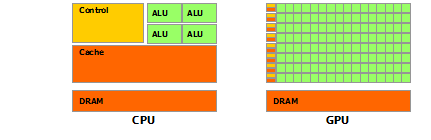
\includegraphics[width=180px]
    {img/device-comparison.png}
}
\end{column}
\end{columns}
\end{frame}

\begin{frame}
\frametitle{Programming GPUs}
\pause
Scientific applications use GPUs at various levels:
\begin{itemize}
    \item Low-level
        \begin{itemize}
            \item CUDA
            \item OpenCL
        \end{itemize}
    \item High-level
        \begin{itemize}[<+->]
            \item OpenACC compiler directives
            \item Drop-in support for scientific libraries such as Intel MKL, BLAS
        \end{itemize}
    \item Transparent
        \begin{itemize}[<+->]
            \item MATLAB: over 200 functions
            \item Software packages: Abaqus, ANSYS (Mechanical/Fluent)
        \end{itemize}
\end{itemize}
\end{frame}

\begin{frame}
\frametitle{CUDA programming model}
\pause
\begin{columns}
\begin{column}{0.5\textwidth}
\textbf{Kernels}
\begin{itemize}[<+->]
    \item Special pieces of code that execute on the GPU
    \item In Fortran: subroutines; in C: functions
    \item Executed concurrently by several GPU threads
\end{itemize}
\textbf{Threads}
\begin{itemize}[<+->]
    \item Threads organized into a grid of blocks
    \item Kernels launched with specified grid size
        (number of blocks) and block size (threads per block)
    \item Grid and blocks can be 2-D or 3-D for convenience
\end{itemize}
\end{column}
\begin{column}{0.5\textwidth}
    \only<5-6>{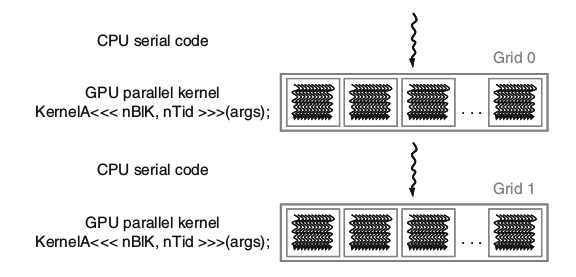
\includegraphics[width=150px]{img/program-structure.png}}
    \only<7>{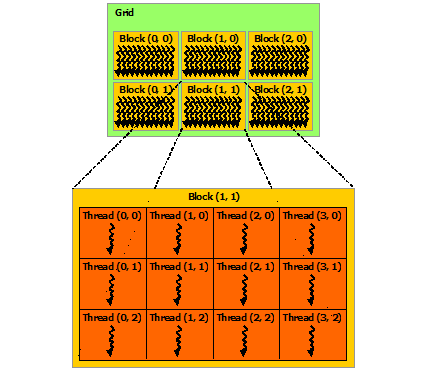
\includegraphics[width=150px]{img/grid-of-thread-blocks.png}}
\end{column}
\end{columns}
\end{frame}

\begin{frame}
\frametitle{GPU architecture and memory model}
\pause
\begin{columns}
\begin{column}{0.5\textwidth}
\begin{itemize}[<+->]
    \item GPU viewed as a collection of \emph{streaming microprocessors} (SMs)
    \item When kernel is launched, each block gets assigned to an SM
    \item Threads within a block execute concurrently
    \item SM may execute several blocks concurrently
\end{itemize}
\end{column}
\begin{column}{0.5\textwidth}
    \visible<3->{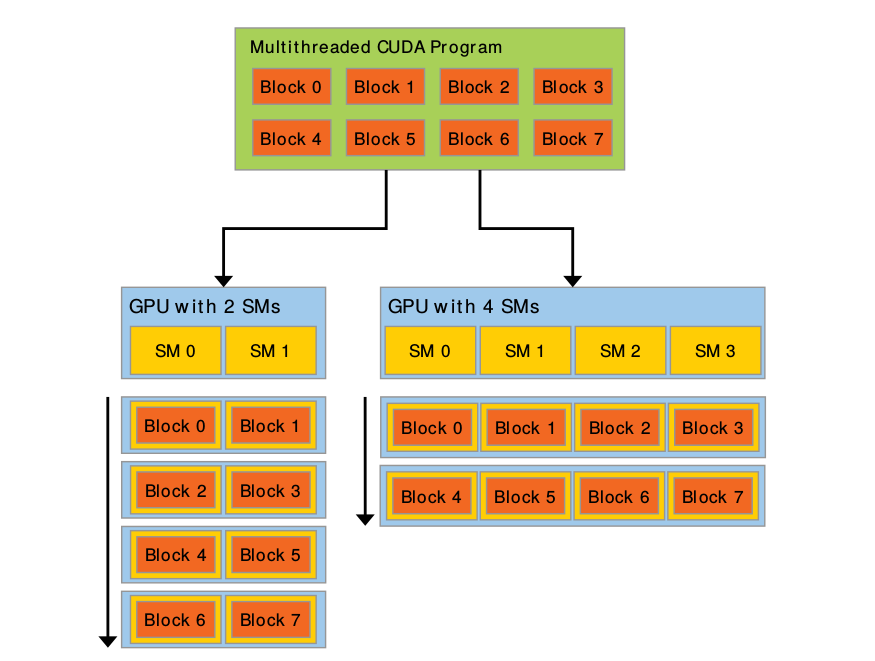
\includegraphics[width=150px]{img/gpu-scaling.png}}
\end{column}
\end{columns}
\end{frame}

\begin{frame}
\frametitle{GPU architecture and memory model}
\pause
\begin{columns}
\begin{column}{0.5\textwidth}
\begin{itemize}
    \item Global memory{
        \begin{itemize}
            \item large but slow (~5 GB for Tesla K20)
            \item all threads can access
            \item persists between kernel launches
        \end{itemize}}
    \item Shared memory{
        \begin{itemize}
            \item small but fast (~48 KiB per SM)
            \item local to threads within a block
            \item explicitly managed cache
        \end{itemize}}
    \item Registers{
        \begin{itemize}
            \item limited (65536 per SM)
            \item local to individual threads
            \item fastest
        \end{itemize}}
\end{itemize}
\end{column}
\begin{column}{0.5\textwidth}
    \visible<2->{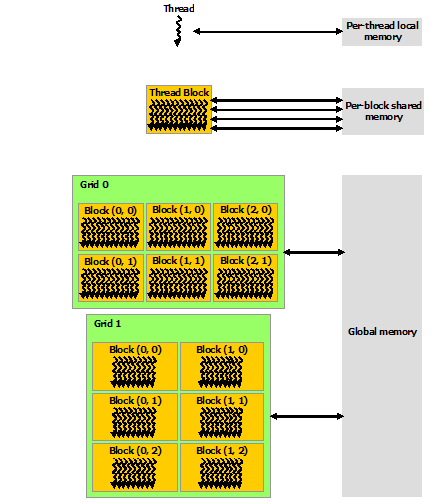
\includegraphics[width=150px]{img/memory-hierarchy.png}}
\end{column}
\end{columns}
\end{frame}


\section{Developing a GPU tridiagonal solver}

\begin{frame}
\frametitle{Requirements of tridiagonal solver}
\begin{columns}
\begin{column}{0.5\textwidth}
\begin{itemize}
\item For a 1-D grid, solution gives the derivative
    at all points simultaneously
\item For 2-D and 3-D grids,
    must solve many independent tridiagonal systems
\item Systems have the same tridiagonal coefficients,
    different right hand sides
\item Need a tridiagonal solver that solves
    a given system for several right hand sides
\item For 2-D problems $n \sim N_{rhs}$;
    for 3-D problems $n << N_{rhs}$
\end{itemize}
\end{column}
\begin{column}{0.5\textwidth}
    \hspace{1cm}
    \includegraphics[width=120px]{img/grid-lines.eps}
\end{column}
\end{columns}
\end{frame}

\begin{frame}
\frametitle{Thomas algorithm}
\begin{itemize}
\item Derived from Gaussian elimination
\item Requires $2n$ steps and $4n$ storage
\item The most efficient sequential algorithm
\item What about parallelization/GPUs?
    \begin{itemize}
        \item inherently sequential
        \item use multiple threads to solve
            individual tridiagonal systems
            (Sakharnykh et al.)
    \end{itemize}
\end{itemize}
\end{frame}

\begin{frame}
\frametitle{Issues in GPU implementation}
\begin{columns}
\begin{column}{0.5\textwidth}
\begin{itemize}
    \item Uncoalesced memory accesses
    \item Needs data rearrangement to coalesce accesses
    \item Does not expose enough parallelism
    \item $2n$ steps - can do better on GPU
    \item A case in which \emph{algorithm choice
        significantly impacts GPU performance}
\end{itemize}
\end{column}
\begin{column}{0.5\textwidth}
    \includegraphics[width=120px]{img/pThomas.eps}
\end{column}
\end{columns}
\end{frame}

\begin{frame}
\frametitle{Tridiagonal solvers for the GPU}
\begin{itemize}
\item Zhang et al. (2010) describe the implementation
    of three algorithms for tridiagonal systems on GPUs
    \begin{itemize}
        \item Cyclic reduction
        \item Parallel cyclic reduction
        \item Recursive doubling
    \end{itemize}
\item \textbf{Step efficient}: trade more work per step for \emph{fewer steps}
\item Exhibit \emph{fine-grained} parallelism - more suited to GPU
\item Subsequent efforts based on CR and PCR primarily
\end{itemize}
\end{frame}

\begin{frame}
\frametitle{Cyclic reduction}
\begin{columns}
\begin{column}{0.5\textwidth}
\begin{itemize}
\item Buzbee and Goleb (1970)
\item \textbf{Forward reduction} ($log_2(n)-1$ steps):
    \begin{itemize}
    \item Eliminate odd-indexed equations at each step
    \item Two-by-two system is left
    \end{itemize}
\item \textbf{Backward substitution} ($log_2(n)-1$ steps):
    \begin{itemize}
    \item Solve for odd-indexed equations using even-indexed values
    \end{itemize}
\item Best case ($n$ parallel threads): requires $2log_2(n)-1$ steps
\end{itemize}
\end{column}
\begin{column}{0.5\textwidth}
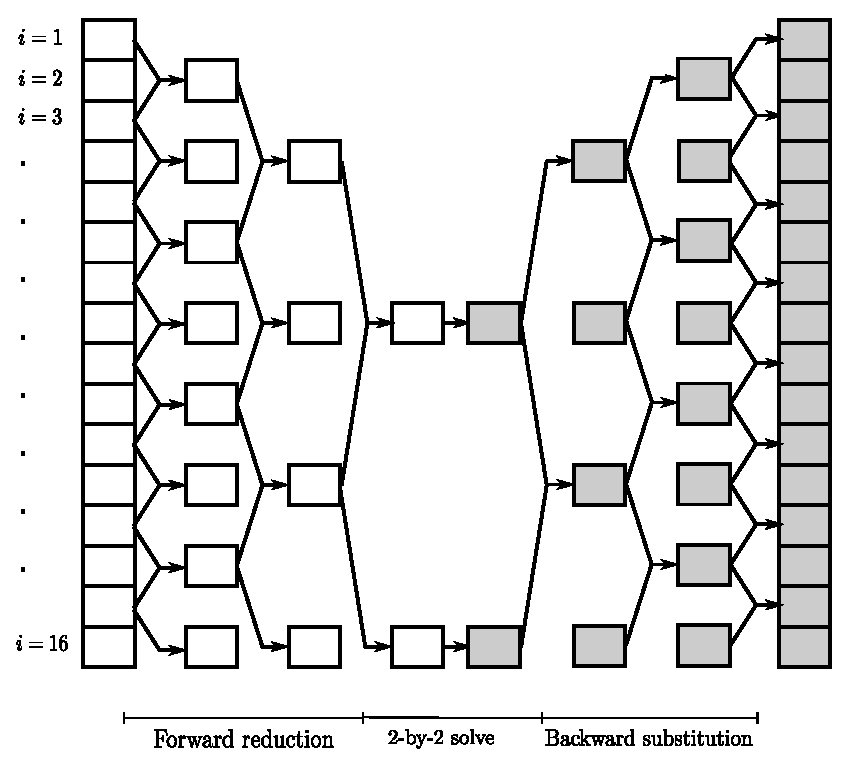
\includegraphics[width=150px]{img/cyclic-reduction.eps}
\end{column}
\end{columns}
\end{frame}

\begin{frame}
\frametitle{Cyclic reduction}
\begin{columns}
\begin{column}{0.5\textwidth}
\begin{itemize}
\item $17n$ operations,
    compared to $8n$ in Thomas algorithm
\item But exhibits more parallelism:
\begin{itemize}
    \item Individual systems can be solved independently
    \item Individual equations can be computed independently
\end{itemize}
\item Equations updated in place: $4n$ storage (same as Thomas algorithm)
\item Synchronization between threads required at each step
\end{itemize}
\end{column}
\begin{column}{0.5\textwidth}
\centering
Forward reduction

(diagonals $a$, $b$, $c$ and RHS $d$)
\scalebox{0.8}{
\vbox{
\begin{align*} 
    k_1 &= \frac{a_i}{b_{i-1}}, k_2 = \frac{c_i}{b_{i+1}} \\
    a^{\prime}_i &= -a_{i-1}k_1 \\
    b^{\prime}_i &= b_i - c_{i-1}k_1 - a_{i+1}k_2 \\
    c^{\prime}_i &= -c_{i+1}k_2 \\
    d^{\prime}_i &= d_i - d_{i-1}k_1  - d_{i+1}k_2 \\
\end{align*}}}

\centering
Backward substitution
\scalebox{0.8}{
\vbox{
\begin{align*}
x_i &= \frac{d^{\prime}_i - a^{\prime}_ix_{i-1} - \
    c^{\prime}_ix_{i+1}}{b^{\prime}_i}
\end{align*}}}
\end{column}
\end{columns}
\end{frame}

\begin{frame}
\frametitle{Issues in GPU implementation}
\footnotesize
\begin{columns}
\begin{column}{0.5\textwidth}
\begin{itemize}
    \item Strided memory access:
        stride increases by a factor of 2 at each step
        (decreases during backward substitution)
    \item \textbf{Solution}: use \emph{shared memory} (cache)
    \item Thread activity decreases during forward
        reduction and increases during backward substitution
    \item \textbf{Solution}: schedule threads for each step
        \begin{itemize}
            \footnotesize
            \item conflicts with shared memory usage
        \end{itemize}
    \item Shared memory \emph{bank conflicts}
        due to power-of-2 strides; reduced GPU occupancy
    \item We provide both implementations:
        global memory \emph{and} shared memory
\end{itemize}
\end{column}
\begin{column}{0.5\textwidth}
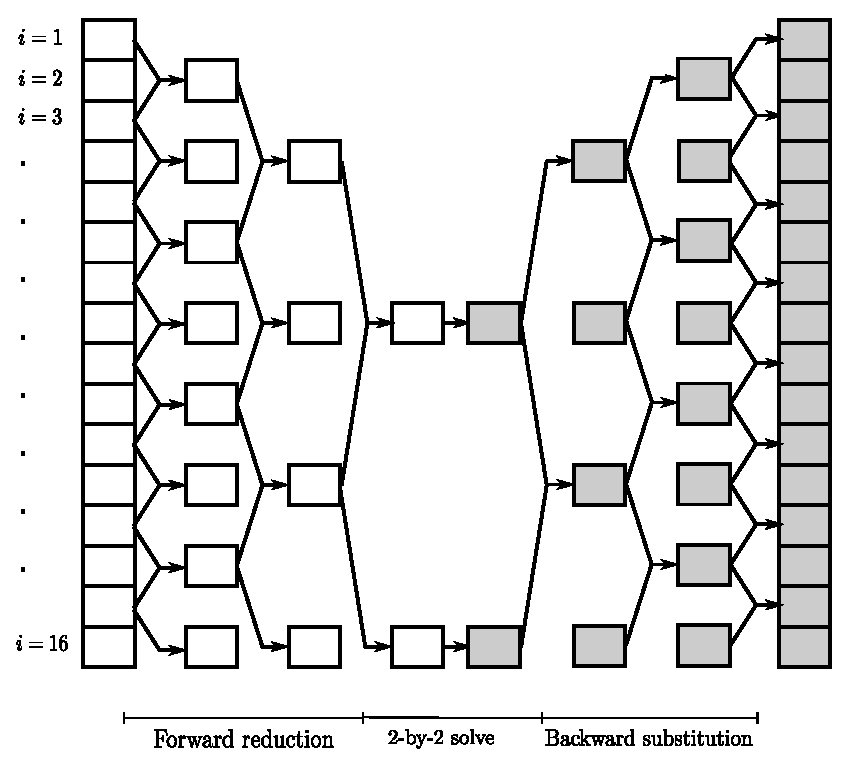
\includegraphics[width=150px]{img/cyclic-reduction.eps}
\end{column}
\end{columns}
\end{frame}

\begin{frame}
\frametitle{Efforts for improving performance}
\begin{itemize}
    \item Zhang et al.: hybrid CR+PCR solver
    \item G{\"o}ddeke et al.: separate even and odd indexed
        coefficients
    \item Davidson et al.: register packing
    \item Esfahanian et al.: global memory with data rearrangement
\end{itemize}
\end{frame}

\begin{frame}
\frametitle{A novel approach}
\begin{columns}
\begin{column}{0.5\textwidth}
\begin{itemize}
\item Solving system with same matrix and different RHS
\item Computing $a^\prime$, $b^\prime$ and $c^\prime$
    for each system and at every time step - \textbf{redundant}
\item Storing coefficients (similar to LU) - \textbf{expensive}
\item Approach: exploit the simple matrix structure
\end{itemize}
\end{column}
\begin{column}{0.5\textwidth}
\centering
Forward reduction
\scalebox{0.8}{
\vbox{
\begin{align*} 
    k_1 &= \frac{a_i}{b_{i-1}}, k_2 = \frac{c_i}{b_{i+1}} \\
    a^{\prime}_i &= -a_{i-1}k_1 \\
    b^{\prime}_i &= b_i - c_{i-1}k_1 - a_{i+1}k_2 \\
    c^{\prime}_i &= -c_{i+1}k_2 \\
    d^{\prime}_i &= d_i - d_{i-1}k_1  - d_{i+1}k_2 \\
\end{align*}}}
\end{column}
\end{columns}
\end{frame}

\begin{frame}
\frametitle{A novel approach}
\begin{columns}
\begin{column}{0.5\textwidth}
\begin{itemize}
\item Diagonals are nearly constant (\emph{near-Toeplitz tridiagonal})
\item Symmetry broken by boundary conditions
\item Near-Toeplitz trdiagonal matrices occur in other numerical schemes
\begin{itemize}
    \item Alternating direct implicit methods
    \item Line relaxation methods
    \item Poisson solvers
    \item One-dimensional ODEs and PDEs
\end{itemize}
\item Can be stored compactly compared to general tridiagonal systems
\end{itemize}
\end{column}
\begin{column}{0.5\textwidth}
\centering
\scalebox{0.6}{%
\vbox{
\begin{equation*}
\begin{bmatrix}
     1&2\\
     1/4&1&1/4\\
     &1/4&1&1/4\\
     &&1/4&1&1/4\\
     &&&1/4&1&1/4\\
     &&&&&\ddots\\
     &&&&&&\ddots\\
     &&&&&&&\ddots\\
     &&&&&&&2&1
  \end{bmatrix}
\end{equation*}}}
\end{column}
\end{columns}
\end{frame}

\begin{frame}
\frametitle{General approach}
\begin{columns}
\begin{column}{0.5\textwidth}
\begin{itemize}
\item Each forward reduction step reduces
    a matrix of size $n$ to $n/2$
\item {First reduction step: substitute:
    \scalebox{0.8}{
    \vbox{
    \begin{align*}
        a_2 &= a_3 = a_4 = \hdots &\equiv a_0 \\
        b_2 &= b_3 = b_4 = \hdots &\equiv b_0 \\
        c_2 &= c_3 = c_4 = \hdots &\equiv c_0
    \end{align*}}}}
\item \textbf{The resulting reduced system is also near-Toeplitz}
\item Each subsequent forward reduction step produces a near-Toeplitz
    tridiagonal system
\begin{itemize}
    \item can be stored compactly
    \item no need to compute for each RHS/time step
\end{itemize}
\end{itemize}
\end{column}
\begin{column}{0.5\textwidth}
\centering
Forward reduction
\scalebox{0.8}{
\vbox{
\begin{align*} 
    k_1 &= \frac{a_i}{b_{i-1}}, k_2 = \frac{c_i}{b_{i+1}} \\
    a^{\prime}_i &= -a_{i-1}k_1 \\
    b^{\prime}_i &= b_i - c_{i-1}k_1 - a_{i+1}k_2 \\
    c^{\prime}_i &= -c_{i+1}k_2 \\
    d^{\prime}_i &= d_i - d_{i-1}k_1  - d_{i+1}k_2 \\
\end{align*}}}
\end{column}
\end{columns}
\end{frame}

\begin{frame}
Cyclic reduction reduced to:

\vspace{1cm}

\textbf{Forward reduction}

\hspace{3.85cm} \sout{$k_1 = \frac{a_i}{b_{i-1}}, k_2 = \frac{c_i}{b_{i+1}}$}

\hspace{3.85cm} \sout{$a^{\prime}_i = -a_{i-1}k_1$}

\hspace{3.85cm} \sout{$b^{\prime}_i = b_i - c_{i-1}k_1 - a_{i+1}k_2$}

\hspace{3.85cm} \sout{$c^{\prime}_i = -c_{i+1}k_2$} 
\begin{align*}
d^{\prime}_i = d_i - d_{i-1}k_1^{m}  - d_{i+1}k_2^{m}
\end{align*}

\textbf{Backward substitution}
\begin{align*}
x_i = \frac{d^{\prime}_i - a^mx_{i-1} - \
    c^{m}x_{i+1}}{b^m}
\end{align*}

where $k_1^m$, $k_2^m$, $a^m$, $b^m$ and $c^m$ are the precomputed
coefficients for $i>1$ at the step $m$.
\end{frame}


\iffalse
\begin{frame}
\frametitle{Finite difference methods}
\pause
\begin{itemize}[<+->]
    \item <2-> Method for solving ordinary and
        partial differential equations
    \item <3-> Approximates the derivatives
        appearing in the equations
        by \emph{finite-difference} approximations
    \item <4-> Two types of derivatives:
    \begin{itemize}
        \item <5-> Spatial
        \item <6-> Temporal
    \end{itemize}
\end{itemize}

\onslide<4-> {
\begin{equation*}
    \alert<6>{\frac{\partial T}{\partial t}} = \alpha (\alert<5>{\frac{\partial^2 T}{\partial x^2}} + \
        \alert<5>{\frac{\partial^2 T}{\partial y^2}})
\end{equation*}
}
\end{frame}

\begin{frame}[t]
\frametitle{Finite difference approximation}
Finite difference approximation of the
first derivative of a uniformly sampled function
\begin{figure}
\includegraphics[width=120px]{img/discretize-function.eps}
\caption{Function $f(x)$, sampled with sampling width $dx$}
\end{figure}
\end{frame}

\begin{frame}[t]
\frametitle{Finite difference approximation}
At sample point $i$,
various approaches for approximating the first derivative:
\begin{columns}[c]
\visible<2->{
    \begin{column}[T]{3cm}
    \begin{figure}
    \includegraphics[width=100px]{img/forward-difference.eps}
    \caption{\textbf{Forward difference}:
        derivative expressed in terms of function values
        at $i$, $i+1$, $i+2$, $\hdots$
    }
    \end{figure}
    \end{column}
}

\visible<3->{
    \begin{column}[T]{3cm}
    \begin{figure}
    \includegraphics[width=100px]{img/backward-difference.eps}
    \caption{\textbf{Backward difference}:
        derivative expressed in terms of function values
        at $\hdots$, $i-2$, $i-1$, $i$
    }
    \end{figure}
    \end{column}
}

\visible<4->{
    \begin{column}[T]{3cm}
    \begin{figure}
    \includegraphics[width=100px]{img/central-difference.eps}
    \caption{\textbf{Central difference}:
        derivative expressed in terms of function values
        at $\hdots$, $i-2$, $i-1$, $i$, $i+1$, $i+2$, $\hdots$
    }
    \end{figure}
    \end{column}
}
\end{columns}
\end{frame}

\begin{frame}[fragile]
\frametitle{Explicit finite difference schemes}
\pause
\begin{itemize}[<+->]
\item The schemes are \emph{explicit}
    because the derivative at each point $i$
    can be expressed \emph{explicitly}
    as some combination of function values
\item Easy to implement in code:
\end{itemize}
\end{frame}

\begin{frame}[t]
\frametitle{Finite difference stencils}
\footnotesize

\begin{block}
{Second order accurate central finite difference scheme} 
\begin{equation*}
    f_i^\prime = \frac{f_{i+1} - f_{i-1}}{2dx}
\end{equation*}
\centering
\includegraphics[width=150px]{img/second-order-stencil.eps}
\end{block}

\begin{block}
{Fourth order accurate central finite difference scheme}
\begin{equation*}
    f_i^\prime = \frac{-f_{i+2} + 4f_{i+1} - 4f_{i-1} +f_{i-2}}{12dx}
\end{equation*}
\centering
\includegraphics[width=150px]{img/fourth-order-stencil.eps}
\end{block}
\end{frame}

\begin{frame}

\end{frame}


\begin{frame}
\frametitle{Parallel computation of finite differences}
\only<1> {
    One dimensional grid of $n$ points:
    \begin{figure}
    \centering
    \includegraphics[width=200px]{img/long-1d-domain.eps}
    \end{figure}
}
\only<2> {
    Split the domain among two parallel processes:
    \begin{figure}
    \centering
    \includegraphics[width=200px]{img/long-1d-domain-split.eps}
    \end{figure}
}
\only<3> {
    Each process can easily compute the derivative at its ``inner points'':
    \begin{figure}
    \centering
    \includegraphics[width=150px]{img/local-derivative-evaluation-inner.eps}
    \end{figure}
}
\only<4> {
    At the process boundaries, communication may be required:
    \begin{figure}
    \centering
    \includegraphics[width=200px]{img/local-derivative-evaluation-boundary.eps}
    \end{figure}
}
\only<5> {
    For a 2-D domain, communication required at each grid line:
    \begin{figure}
    \centering
    \includegraphics[width=200px]{img/local-derivative-evaluation-boundary-2d.eps}
    \end{figure}
}
\only<6> {
    Amount of communication grows with problem dimensionality and stencil width:
    \begin{figure}
    \centering
    \includegraphics[width=200px]{img/overall-halos.eps}
    \end{figure}
}
\end{frame}

\begin{frame}
\begin{itemize}[<+->]
    \item Explicit finite difference schemes are simple to implement
    \item Higher order accurate schemes require wider stencils
    \item Reduces the compute to communicate ratio in parallel
\end{itemize}
\end{frame}

\begin{frame}
\frametitle{Compact finite difference schemes}
\begin{itemize}[<+->]
    \item High order of accuracy for smaller stencil widths
    \item Express the derivative \emph{implicitly}:
    \item [] \begin{align*}
        \begin{split}
            f_i^{\prime} + \alpha(f^{\prime}_{i-1} + f^{\prime}_{i+1}) + \
            \beta(f^{\prime}_{i-2} + f^{\prime}_{i+2}) + \hdots  = \
            a\frac{f_{i+1} - f_{i-1}}{dx} + \\
            b\frac{f_{i+2} - f_{i-2}}{dx} + \
            c\frac{f_{i+3} - f_{i-3}}{dx} + \
            \hdots
        \end{split}
        \end{align*}
\end{itemize}
\end{frame}

\begin{frame}
\footnotesize
\begin{align*}
\begin{split}
    f_i^{\prime} + \alpha(f^{\prime}_{i-1} + f^{\prime}_{i+1}) + \
    \beta(f^{\prime}_{i-2} + f^{\prime}_{i+2}) + \hdots = \
    a\frac{f_{i+1} - f_{i-1}}{h} + \\
    b\frac{f_{i+2} - f_{i-2}}{h} + \
    c\frac{f_{i+3} - f_{i-3}}{h} + \
    \hdots
\end{split}
\end{align*}
\pause
\begin{itemize}
    \item <2-> Difficult to implement compared to explicit schemes
    \item <3-> Consider the scheme with
        $\alpha=\frac{1}{4}$, $\beta=0$, $a=\frac{3}{4}$,
        $b=c=\hdots=0$:
    \item <4-> For $i = 2, 3, \hdots .. n-1$:
\end{itemize}
\begin{align*}
\onslide<5->{f_2^{\prime} + \frac{1}{4}(f^{\prime}_{1} + f^{\prime}_{3}) =
    \frac{3}{4}\frac{f_{3} - f_{1}}{dx}} \\
%
\onslide<6->{f_3^{\prime} + \frac{1}{4}(f^{\prime}_{2} + f^{\prime}_{4}) =
    \frac{3}{4}\frac{f_{4} - f_{2}}{dx} \\}
%
\onslide<7->{f_4^{\prime} + \frac{1}{4}(f^{\prime}_{3} + f^{\prime}_{5})
    = \frac{3}{4}\frac{f_{5} - f_{3}}{dx} \\}
%
\onslide<8->{\hdots}
\onslide<8->{f_{n-1}^{\prime} + \frac{1}{4}(f^{\prime}_{n-2} + f^{\prime}_{n})
    = \frac{3}{4}\frac{f_{n} - f_{n-2}}{dx}}
\end{align*}
\end{frame}

\begin{frame}
\begin{itemize}
    \item Special equations required to close the boundaries
    \item Boundary equations have the following general form:
        \begin{equation*}
            f_1^{\prime} + \alpha^{\prime}f_2^{\prime} = \
                \frac{1}{h}(a^{\prime}f_1 + b^{\prime}f_2 + \
                    c^{\prime}f_3 + d^{\prime}f_4)
        \end{equation*}
    \item Consider the following boundary scheme 
        \begin{align*}
            f^{\prime}_1 + 2f^{\prime}_2 &= \frac{-5f_1 + 4f_2 + f_3}{dx} \\
            f^{\prime}_{n} + 2f^{\prime}_{n-1}
            &=
            \frac{5f_{n} - 4f_{n-2} -  f_{n-1}}{dx}
        \end{align*}
\end{itemize}
\end{frame}

\begin{frame}
\footnotesize
The full set of equations is:
\begin{align*}
    f^{\prime}_1 + 2f^{\prime}_2 &= \frac{-5f_1 + 4f_2 + f_3}{dx} \\
    %
    f_2^{\prime} + \frac{1}{4}(f^{\prime}_{1} + f^{\prime}_{3}) &=
        \frac{3}{4}\frac{f_{3} - f_{1}}{dx} \\
    %
    f_3^{\prime} + \frac{1}{4}(f^{\prime}_{2} + f^{\prime}_{4}) &=
        \frac{3}{4}\frac{f_{4} - f_{2}}{dx} \\
    %
    f_4^{\prime} + \frac{1}{4}(f^{\prime}_{3} + f^{\prime}_{5}) &=
        \frac{3}{4}\frac{f_{5} - f_{3}}{dx} \\
    %
    \hdots& \\
    %
    f_{n-1}^{\prime} + \frac{1}{4}(f^{\prime}_{n-2} + f^{\prime}_{n}) &=
        \frac{3}{4}\frac{f_{n} - f_{n-2}}{dx} \\
    %
    f^{\prime}_{n} + 2f^{\prime}_{n-1} &=
        \frac{5f_{n} - 4f_{n-2} -  f_{n-1}}{dx}
\end{align*}
\end{frame}

\begin{frame}
\footnotesize
Can be expressed as a system of equations:
\begin{equation*}
 \begin{bmatrix}
     1&2\\
     1/4&1&1/4\\
     &1/4&1&1/4\\
     &&1/4&1&1/4\\
     &&&1/4&1&1/4\\
     &&&&&\ddots\\
     &&&&&&\ddots\\
     &&&&&&&\ddots\\
     &&&&&&&2&1
  \end{bmatrix}
  \begin{bmatrix}
      f^{\prime}_1 \\

      f^{\prime}_2 \\
      f^{\prime}_3 \\
      \vdots \\
      \vdots \\
      \vdots \\
      \vdots \\
      f^{\prime}_{n-1} \\
      f^{\prime}_n
   \end{bmatrix}
 =
 \begin{bmatrix}
     \frac{-5f_1 + 4f_2 + f_3}{2dx}\\
     \frac{3(f_{3} - f_{1})}{4dx}\\
     \frac{3(f_{4} - f_{2})}{4dx}\\
     \vdots\\
     \vdots\\
     \vdots\\
     \vdots\\
     \frac{3(f_{n} - f_{n-2})}{4dx}\\
     \frac{5f_{n} - 4f_{n-1} - f_{n-2}}{2dx}
  \end{bmatrix}
\end{equation*}

\pause
\begin{itemize}[<+->]
    \item The derivatives at $i=1,2, .. n$ are solved \emph{simultaneously}
    \item In general, this requires solution of a \emph{banded} linear system
\end{itemize}
\end{frame}


\begin{frame}
\frametitle{The need for parallel systems}
\pause
\begin{itemize}[<+->]
    \item Computation established as the ``third route''
        to scientific truth
    \item Solving real problems:
        energy research,
        climate modeling,
        protein folding,
        quantum mechanics...
    \item Computational \emph{power} soon becomes
        the bottleneck for the size and scope of
        problems that can be solved
    \item 2003 famously quoted as the end
        of the monolithic processor;
        parallel computing synonymous with
        high-performance computing
\end{itemize}
\end{frame}

\begin{frame}[shrink=20,t]
\frametitle{The workhorses of scientific computation}
\pause
\begin{columns}[T]
\visible<2->{
\begin{column}{0.33\textwidth}
\textbf{Multi-core CPU}
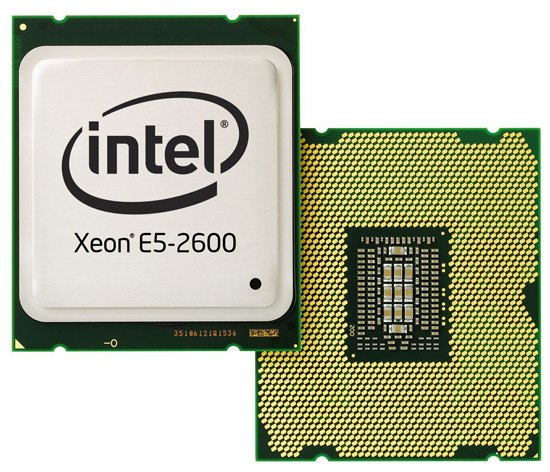
\includegraphics[width=100px]{img/intel-xeon-device.jpg}
\begin{itemize}
    \item<5-> 2-16 cores
    \item<6-> General-purpose computation
    \item<7-> Programming: OpenMP, PThreads, MPI
    \item<8-> Focus of vast majority of scientific
        software
\end{itemize}
\end{column}
}

\visible<3->{
\begin{column}{0.33\textwidth}
\textbf{Many-core GPU}
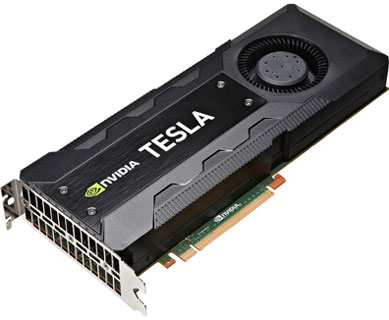
\includegraphics[width=100px]{img/tesla-k20-device.jpg}
\begin{itemize}
    \item<9-> Hundreds of compute cores
    \item<10-> \emph{Massively-parallel} computations
    \item<11-> Programming: CUDA, OpenCL
    \item<12-> Supported by major packages,
        proven for several applications
\end{itemize}
\end{column}
}

\visible<4->{
\begin{column}{0.33\textwidth}
\textbf{Intel Many Integrated Core \emph{coprocessor}}
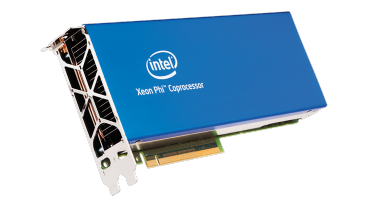
\includegraphics[width=120px]{img/xeon-phi-device.png}
\begin{itemize}
    \item<13-> 50-72 cores
    \item<14-> Require more parallelism to reach
        peak performance
    \item<15-> CPU-like programmability
    \item<16-> Support by packages is scarce
        but growing
\end{itemize}
\end{column}
}
\end{columns}
\end{frame}

\begin{frame}[t]
\frametitle{Why GPUs?}
\pause
\footnotesize
\begin{columns}[T]
\begin{column}{0.4\textwidth}
\begin{itemize}
    \item<2-> Higher peak performance
        compared to multicore CPUs
    \item<3-> Higher memory bandwidth
    \item<4-> Devotes more resources
        (transistors) to computing
        rather than caching/control flow
    \item<5-> Well-suited to
        highly data-parallel computations---often the
        \emph{kernels} in scientific computation
\end{itemize}
\end{column}

\begin{column}{0.6\textwidth}
\includegraphics<2>[width=180px]
    {img/floating-point-operations-per-second.png}
\includegraphics<3>[width=180px]
    {img/memory-bandwidth.png}
\includegraphics<4>[width=180px]
    {img/device-comparison.png}
\includegraphics<5>[width=180px]
    {img/device-comparison.png}
\end{column}
\end{columns}
\end{frame}


\section{Proposed Tridiagonal Algorithm}
\begin{frame}
\frametitle{Graphics processing units}
\begin{columns}[c]
\begin{column}[T]{5cm}
    Expectations
    \begin{figure}
    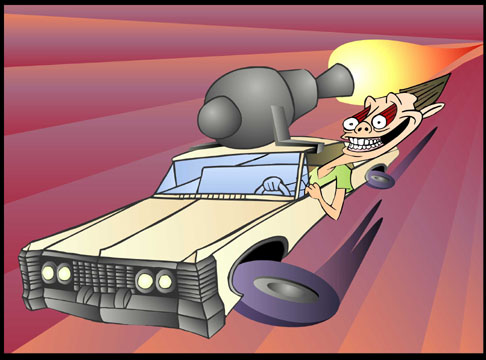
\includegraphics[width=150px]{img/expectations.jpg}
    \end{figure}
\end{column}

\begin{column}[T]{5cm}
    Reality
    \begin{figure}
    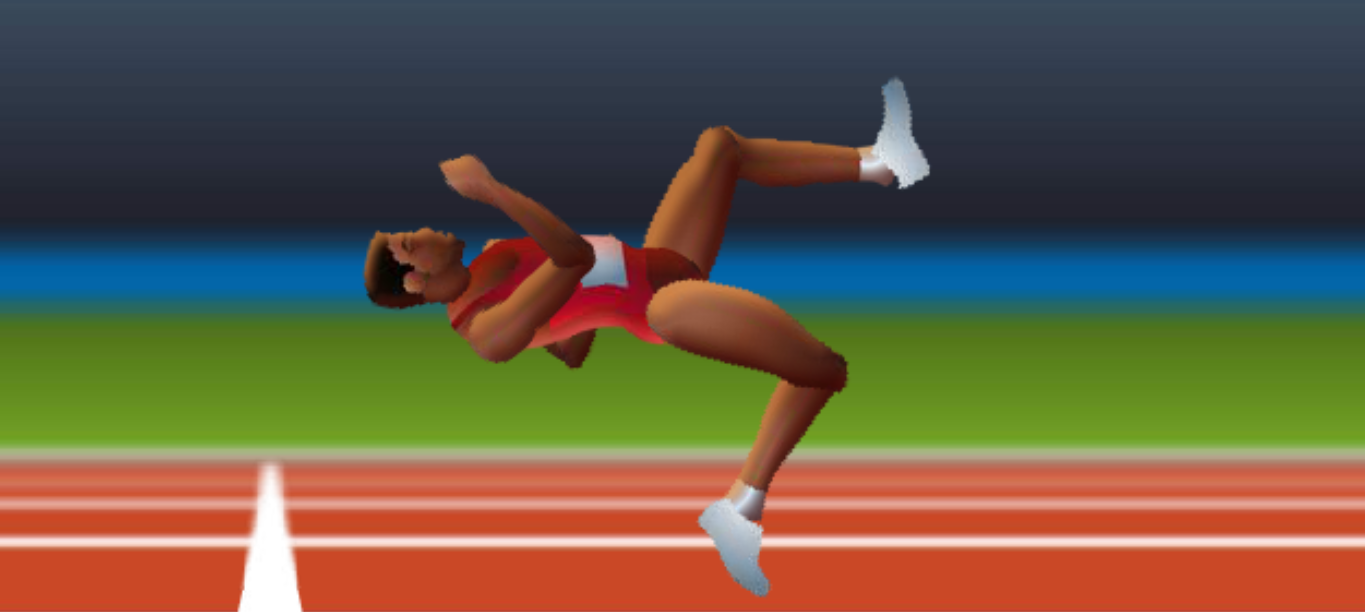
\includegraphics[width=150px]{img/reality.png}
    \end{figure}
\end{column}
\end{columns}
\end{frame}

\section{Distributed Compact Finite Difference Evaluation}
\begin{frame}
\frametitle{Graphics processing units}
\begin{columns}[c]
     \begin{column}[T]{5cm}
        Expectations
        \begin{figure}
        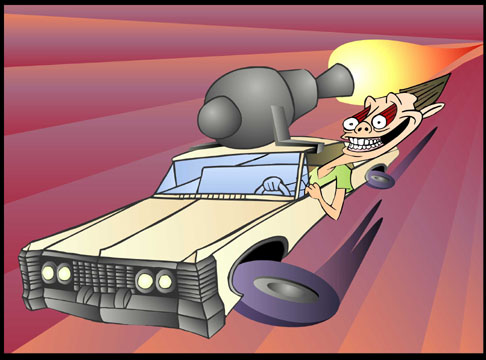
\includegraphics[width=150px]{img/expectations.jpg}
        \end{figure}
    \end{column}

    \begin{column}[T]{5cm}
        Reality
        \begin{figure}
        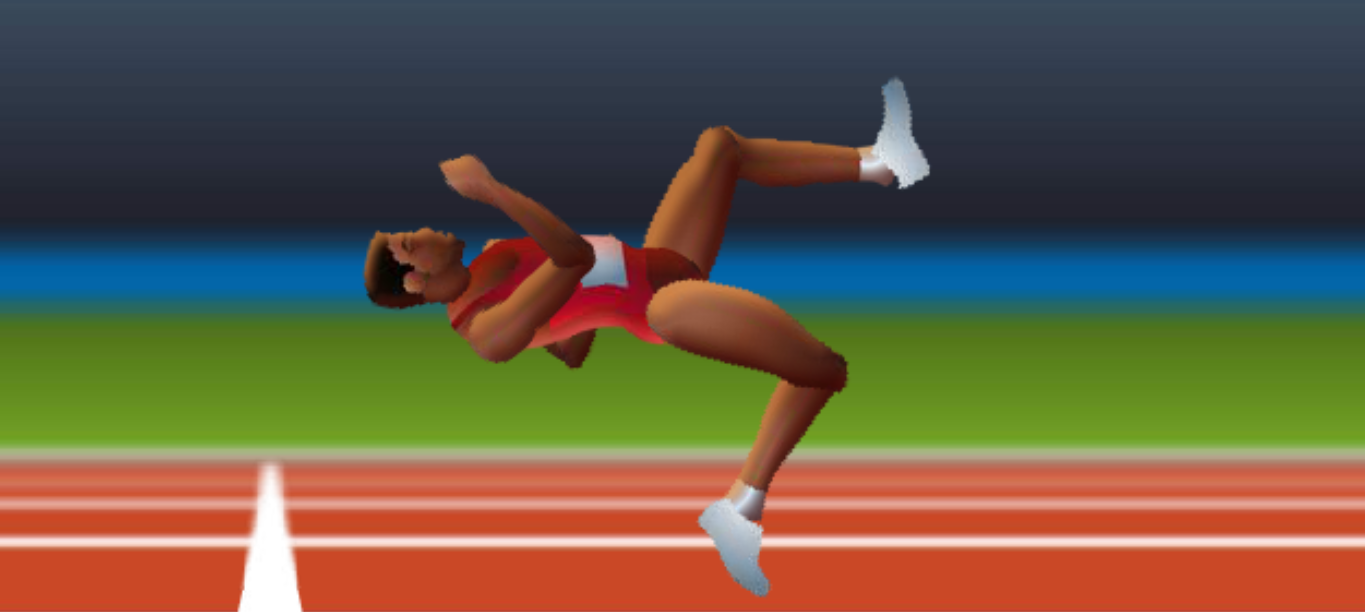
\includegraphics[width=150px]{img/reality.png}
        \end{figure}
    \end{column}
\end{columns}
\end{frame}

\section{Results}

\begin{frame}
\frametitle{Graphics processing units}
\begin{columns}[c]
     \begin{column}[T]{5cm}
        Expectations
        \begin{figure}
        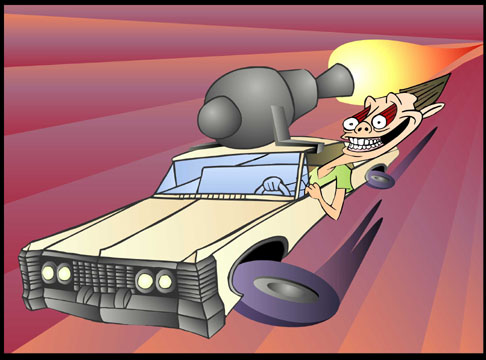
\includegraphics[width=150px]{img/expectations.jpg}
        \end{figure}
    \end{column}

    \begin{column}[T]{5cm}
        Reality
        \begin{figure}
        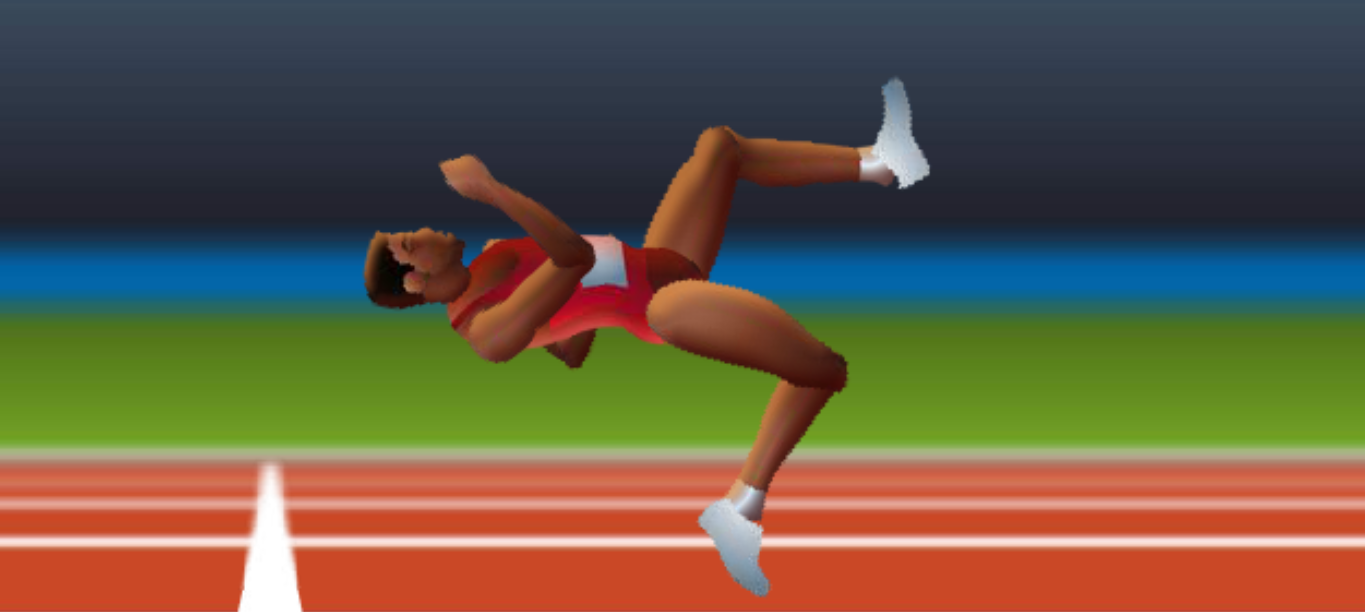
\includegraphics[width=150px]{img/reality.png}
        \end{figure}
    \end{column}
\end{columns}
\end{frame}
\fi

\end{document}

